\chapter{Disseny}
\label{cha:dessign}

En aquest cap\'{i}tol s'explica el disseny implementat per complir l'especificació del sistema. Es defineix la arquitectura del sistema, els patrons de dissenys emprats i les interfícies m\'{e}s complexes. 

\section{Esquema general l\`{o}gic arquitect\'{o}nic del sistema}
A continuació s'explica l'arquitectura lògica dels components del sistema. La figura \ref{fig:archsoftware} a la p\`{a}gina \pageref{fig:archsoftware} \'{e}s un esquema d'aquesta arquitectura. Els components de l'arquitectura son:\\

\begin{figure}[h!]
  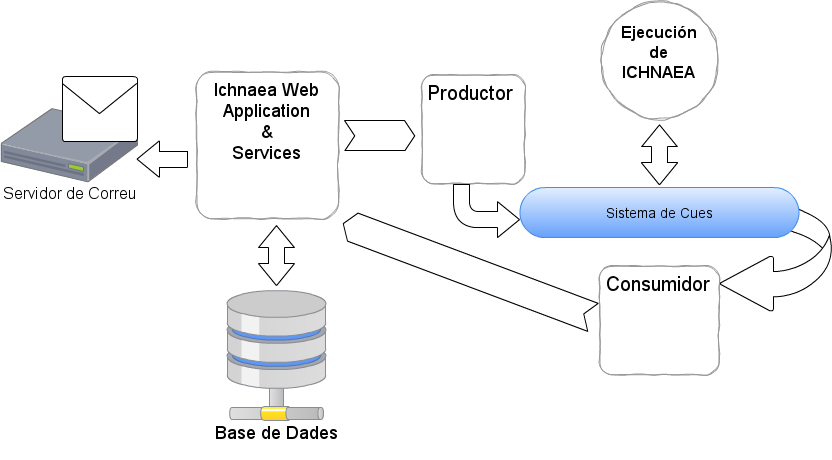
\includegraphics[scale=0.5]{img/design/ArchitectureSoftware.png}
  \caption{Diagrama de l'arquitectura del sistema}
  \label{fig:archsoftware}
\end{figure}

\begin{itemize}
\item \textit{Ichnaea Web Application \& Services}: \'{e}s el \textit{core} de la aplicaci\'{o} i dels serveis HTTP. Es el codi i la aplicació desenvolupada. Es el principal responsable d'aquest projecte.
\item Servidor de correu \'{e}s el servidor SMTP per enviar correus electr\`{o}nics als usuaris.
\item Productor-Cua-Consumidor \'{e}s el sistema de cues. Expliquem el paradigma a la secció \ref{sec:queue_system_overview}. La funci\'{o} \'{e}s gestionar els inicis, fluxos i finals d'execucions de Ichnaea.
\item La base de dades \'{e}s on es guarden els continguts, els models de dades i els resultats.
\item El sistema de fitxers \'{e}s on es guarden els resultats en format binari dels entrenaments per usar amb les prediccions.
\end{itemize}
Es contempla una arquitectura distribuïda com a base inicial per complir els requeriments d'escalabilitat en els casos de augment o disminucions de recursos i per tenir un sistema amb un bon rendiment.\\

A continuació donem una visió global dels patrons usats, de com es distribueixen i de les seves responsabilitats.

\section{Patrons de disseny}
Per la implementaci\`{o} del sistema web s'ha usat un disseny per capes. Les capes son presentaci\'{o}, domini i persistència de dades. S'han seleccionat els següents patrons per complir els requeriments especificats.
  \begin{itemize}
  \item Model-Vista-Controlador amb controlador frontal
  \item Capa de Servei
  \item Injecci\'{o} de depend\`{e}ncies
  \item Repositori de model de dades
  \item Capa de mapejat de dades
  \item View template
  \item Interfícies enriquides amb servei webs
  \end{itemize}
A continuació expliquem detallem cadascun d'aquests patrons.

\subsection{Esquema del disseny}
\label{subsec:dessigndiagram}
Per tal de donar una visió general del patrons de disseny usats, dediquem aquesta secció a un diagrama esquemàtic dels patrons usats degut a la complexitat del disseny.\\

La figura \ref{fig:dessignpatters} a la p\`{a}gina \pageref{fig:dessignpatters} dona una visió general de la distribució dels patrons en els capes i com s'integren.\\
\begin{sidewaysfigure}[ht]
  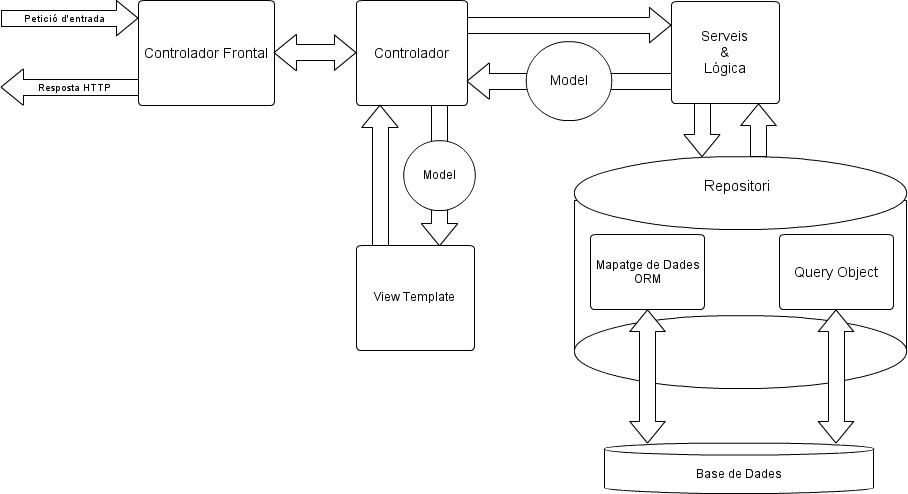
\includegraphics[scale=0.4]{img/design/IchnaeaPatterns.png}
  \caption{Patrons de disseny}
  \label{fig:dessignpatters}
\end{sidewaysfigure}

A continuació expliquem detalladament els patrons de disseny, la integració entre ells i les seves responsabilitats.

\subsection{Explicaci\'{o} del disseny}
\label{subsec:dessignexplanation}

\phantomsection
\label{mvcFrontController}
\subsubsection{Model-Vista-Controlador amb controlador frontal}
El patró Model-Vista-Controlador \'{e}s un disseny t\'{i}pic en les aplicacions web on:
\begin{itemize}
\item el \textbf{model} \'{e}s una representaci\'{o} de les dades.
\item la \textbf{vista} transforma el model a un format visible i llegible.
\item el \textbf{controlador} rep les peticions i dona les sortides.
\end{itemize}
El \textbf{controlador frontal} \'{e}s una variació del controlador que centralitza totes les peticions i les re-dirigeix cap als controladors corresponents m\'{e}s especialitzats.\\

Les principals avantatges d'aquesta variació \'{e}s la centralització de les peticions en un únic punt. Això t\'{e} un impacte directe en l'augment de la re-usabilitat del codi i d'una millor gestió de la seguretat.

\subsubsection{Injecció de dependències}
L'arquitectura \textbf{MVC} separa la capa de presentaci\'{o} de la l\`{o}gica de domini. La capa de presentaci\'{o} accedeix a la capa de domini mitjançant serveis, injectant depend\'{e}ncies (secció \ref{subsec:dessigndiagram}).\\

La \textbf{injecci\'{o} de depend\'{e}ncies} \'{e}s un patr\'{o} a on es subministren objectes a una classe en lloc de ser la classe qui crea els objectes.\cite{dependency_injection}\\

Les avantatges de usar DI(''dependency injection'') son:
\begin{itemize}
\item Codi m\'{e}s f\`{a}cil de mantenir, extendre o modificar.
\item Desenvolupament guiat per proves (Test Driven Development o TDD en angl\'{e}s).
\item DI ens obliga a planejar una mica millor les nostres depend\`{e}ncies; decidim si una classe realment necessita d'un altre objecte per realitzar la seva funció.
\end{itemize}

\subsubsection{Repositori de model de dades}
La \textbf{capa de serveis} cont\'{e} la l\'{o}gica del sistema web d'Ichnaea i depen directament del domini. El domini accedeix a les dades mitjançant \textbf{repositoris} d'objectes. Els \textbf{repositoris} son mediadors entre el domini i les dades persistents. Els repositoris retornen entitats i/o col·leccions d'entitats de la l\'{ogica} de domini.\\

Les principals avantatges d'aquest patró son la facilitat de realitzar tests, la clara segregació entre capa de domini i la capa de dades i la possibilitat de usar els repositoris amb altres dominis.\\

La principal avantatge de la integració entre el patró repositori i la injecció de dependències \'{e}s el \textbf{desacoblament entre domini i la capa de dades}. En altres paraules, es podria canviar la tecnologia de la capa de dades sense fer quasi cap modificació. 

\phantomsection
\label{ormdessign}
\subsubsection{Capa de mapatge de dades}
El \textbf{mapatge de dades} ORM(''Object Relational Mapping'' o mapatge objecte-relacional) \'{e}s un patr\'{o} de disseny(encara que alguns enginyers els agrada dir que \'{e}s una tècnica de programaci\'{o} i a uns altres una tecnologia) que estableix una relaci\'{o} directe entre les entitats i la dades persistents.\cite{orm}\\

Les principals avantatges d'usar aquest patró son la facilitat de desenvolupament, abstracció de la base de dades, la seguretat i el manteniment del codi.\\

En qualsevol projecte es molt útil ja que mentre es desenvolupen les classes, a la vegada es defineixen els esquemes de les bases de dades.

\subsubsection{View template}
El patró de vista ''template'' es una variació del component \textbf{Vista} del patró \textbf{MVC}. Es un patró molt vinculat al desenvolupament de pagines HTML i la entitat base son les plantilles.\\

Les plantilles son pagines estàtiques amb informació dinàmica mitjançant variables. El controlador del patró MVC emplena aquestes variables generant pagines dinàmicament.\cite{viewtemplate}\\

Les principals avantatges d'usar aquest patró son la clara separació entre vistes i lògiques d'aplicació i del controlador.  

\phantomsection
\label{ria}
\subsubsection{Interfícies enriquides amb serveis webs}
Les aplicacions web enriquides(RIA) son aplicacions que tenen la majoria de les funcions de les aplicacions d'escriptori tradicional. L'objectiu es millorar la experiència i la productivitat de l'usuari. En aquest cas, com \'{e}s un sistema web, els clients son els navegadors webs o els perifèrics com altres sistemes o una aplicació mòbil.\cite{ria}\\

L'us del patró ''View Template'' ens facilita que part del desenvolupament de l'aplicació estigui al costat del clients(navegadors) per dissenyar unes interfícies complexes i enriquides.\\ 

\section{Disseny d'interf\'{i}cies}
\label{sec:dessigninterfaces}
En el disseny de les interfícies, es pretén definir com serà la part del sistema que interactua amb l’usuari. Consisteix en definir els mecanismes amb els quals els usuaris podran interactuar amb el sistema i la manera de mostrar la informació a l’usuari.\\

A continuació es detalla el disseny principal de l'aplicació i de les interfícies m\'{e}s complexes.

\subsection{Disseny principal}
\label{subsec:maindessign}
A la figura \ref{fig:maininterface} es detalla la estructura estètica de la aplicació. 

\begin{figure}[H]
  \centering
  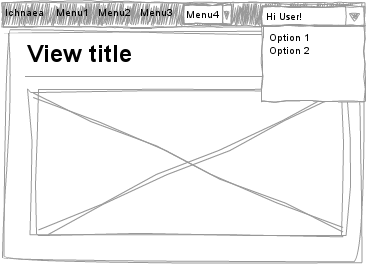
\includegraphics[scale=0.7]{img/design/Maininterface.png}
  \caption{\textit{Disseny tipus ''Wireframe'' de la estructura estètica de la aplicació}}
  \label{fig:maininterface}
\end{figure}

La capçalera de totes les p\`{a}gines del sistema serà sempre visibles i contindrà el menú de la aplicació. A la part esquerra del menu sortira el logo d'Ichnaea i a la dreta un menú per l'usuari.\\

El menú contindrà dos nivell. El primer nivell esta detallat a la capçalera. I el segon nivell es desplegar\'{a} al accedir a la opci\'{o} del primer nivell.\\

\phantonsection
\label{menudessign}
El menú serà condicional als permisos de l'usuari que estigui usant la aplicació. La jerarquia del menú es la següent:
\begin{itemize}
\item Logo
\item Matrius.
 \begin{itemize}
 \item Les meves matrius
 \item Crear una matriu
  \end{itemize}
\item Entrenaments
 \begin{itemize}
 \item Els meus entrenaments
 \item Crear un entrenament
 \end{itemize} 
\item Prediccions
 \begin{itemize}
 \item Les meves prediccions
 \item Crear una predicció
 \end{itemize} 
\item Dades de Ichnaea. Son dades generals consultables per tots els usuaris.
 \begin{itemize}
 \item Variables del sistema
 \item Fitxers
 \item Matrius
 \item Llista de entrenaments predictibles
 \end{itemize} 
\item Administració: Solament disponible per usuaris administradors
\begin{itemize}
\item Usuaris
\item Crear una variable
\item Eines administratives de control de cues
\item Llista d'entrenaments
\item Llista de prediccions
\end{itemize}
\item Usuari
 \begin{itemize}
 \item Casa de l'usuari
 \item Canvi de contrasenya
 \item Desconectar-se
 \end{itemize}
\end{itemize}

\subsection{Interf\'{i}cie de configuraci\'{o} de matrius}
El disseny d'interfícies per les configuracions de les matrius es basa en desenvolupar funcionalitats enriquides\cite{ria}. Per dotar de funcionalitats a les interfícies webs s'utilitza el paradigma de peticions asíncrones;\cite{asyncronous} mitjançant l'aplicació del patró de disseny ''Interfícies enriquides amb serveis webs''(explicat a la secció \ref{subsec:dessignexplanation} a la pagina \pageref{ria}).\\ 

Per complir aquest requeriment s'ha de dissenyar una llibreria per atendre les peticions asíncrones i desenvolupar funcionalitats a les interfícies per atendre les respostes a aquestes peticions. A continuaci\'{o} es descriuen les interf\'{i}cies m\'{e}s complexes que son les de configuraci\'{o} de matrius.

\subsubsection{Interf\'{i}cie de configuraci\'{o} de matrius}
Per tenir una bona experiència de usuari, la interfície de configuració de matrius ha de permetre la configuració de les dades de les matrius de forma asíncrona. La interfície ha de mostrar una graella amb moltes dades. Per tant \'{e}s important separar clarament les dades i les funcionalitats de configuració.\\

Les funcionalitats enriquides que ha de complir la interfície son:
\begin{itemize}
\item Carregar un conjunt de fitxers segons la variable seleccionada.
\item Guardar la configuració d'una columna: alies, variable i conjunt de fitxers.
\item Desplegar un calendari per seleccionar una data i assignar-la a una mostra.
\item Desplegar un selector obert de possibles valors de tots els orígens que estiguin especificats a les mostres.
\item Actualitzar el valor d'una mostra i d'una variable.
\item Permetre la mobilitat per les dades de la matriu fixant les capçaleres de les columnes i les files perquè l'usuari tingui una referencia clara a que correspon la dada.
\item Adaptar-se a les dimensions de la pantalla.
\end{itemize}

A la figura \ref{fig:interfacematrixconf} s'especifica el disseny de la interfície de configuraci\'{o} de matrius. A l'apèndix \ref{cha:userguide} es pot consultar el resultat dels dissenys especificats.

\begin{figure}[H]
  \centering
  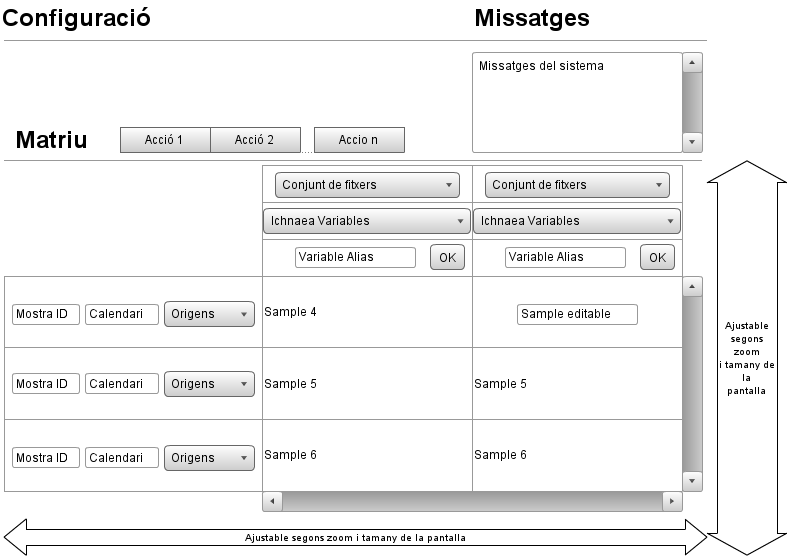
\includegraphics[scale=0.5]{img/design/Interficiedeconfiguracio.png}
  \caption{Interfície de configuració de matrius}
  \label{fig:interfacematrixconf}
\end{figure}


\subsubsection{Interf\'{i}cie de configuraci\'{o} de matrius de predicció}
Al igual que l'anterior, per tenir una bona experiència de usuari, la interfície de configuració de matrius de predicció ha de permetre la configuració de les dades de les matrius de forma asíncrona. La interfície ha de mostrar una graella amb moltes dades. Per tant \'{e}s important separar clarament les dades i les funcionalitats de configuració.\\

Les funcionalitats enriquides que han de complir:
\begin{itemize}
\item Guardar la configuració de una columna: alies i assignació d'una columna entrenada.
\item Desplegar un calendari per seleccionar una data i assignar-la a una mostra.
\item Desplegar un selector obert de possibles valors de tots els orígens que estiguin especificats a les mostres.
\item Actualitzar el valor d'una mostra i d'una variable.
\item Adaptar-se a les dimensions de la pantalla.
\end{itemize}

A la figura \ref{fig:interfacematrixpredictionconf} s'especifica el disseny de la interfície de configuraci\'{o} de matrius de prediccions. A l'apèndix \ref{cha:userguide} es pot consultar el resultat dels dissenys especificats.

\begin{figure}[H]
  \centering
  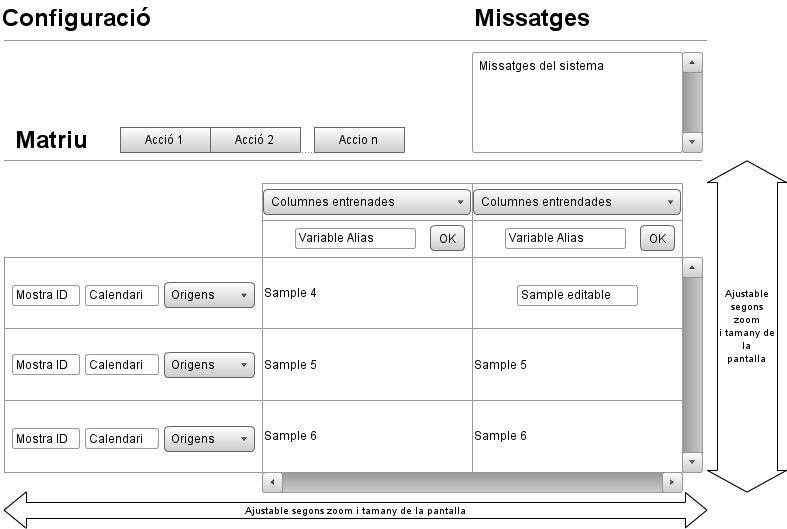
\includegraphics[scale=0.5]{img/design/Interficiedeconfiguraciopredi.png}
  \caption{Interfície de configuració de matrius de prediccions}
  \label{fig:interfacematrixpredictionconf}
\end{figure}
